\chapter{Magma Dynamics: porosity waves}
\label{cha:porosity-waves}

\section{Problem Overview}
\label{sec:porosity_waves-formulation}


While many modeling packages in Earth science solve for thermal or
thermo-chemical convection,  one of the strengths of \TF{} is that it
is not a ``convection code'' or a ``magma code'', but rather a general finite element PDE
solver and can be used to model arbitrary problems as long as the weak
forms are well posed.  In particular,  \TF{} was primarily designed to
explore coupled fluid/solid mechanics with a primary application area
being the flow of magma and fluids in the deep earth.  A more general
theory of magma dynamics has been derived by multiple authors
\cite{mckenzie_generation_1984,scott_magma_1984,scott_magma_1986,spiegelman_flow_1993,spiegelman_flow_1993-1,bercovici_two-phase_2001-1,bercovici_energetics_2003,simpson_multiscale_2010,simpson_multiscale_2010-1}
that considers the flow of a low viscosity fluid in a viscously
deformable solid matrix.  From the beginning of magma dynamics,  one
of the intriguing features of these models is that they admit
dispersive non-linear magmatic
solitary  waves that propagate through the solid as ``hump
shaped'' blobs with radial symmetry that propagate at a characteristic
speed $c$ that depends on amplitude, dimension and material
parameters.  Figure \ref{fig:SolitaryWavesAllD} shows some example
solitary wave profiles for 1,2 and 3-D solitary waves that all
propagate at the same speed $c=5$ times the melt velocity in the
background constant porosity region.  

\begin{figure}[htb!]
  \centering
  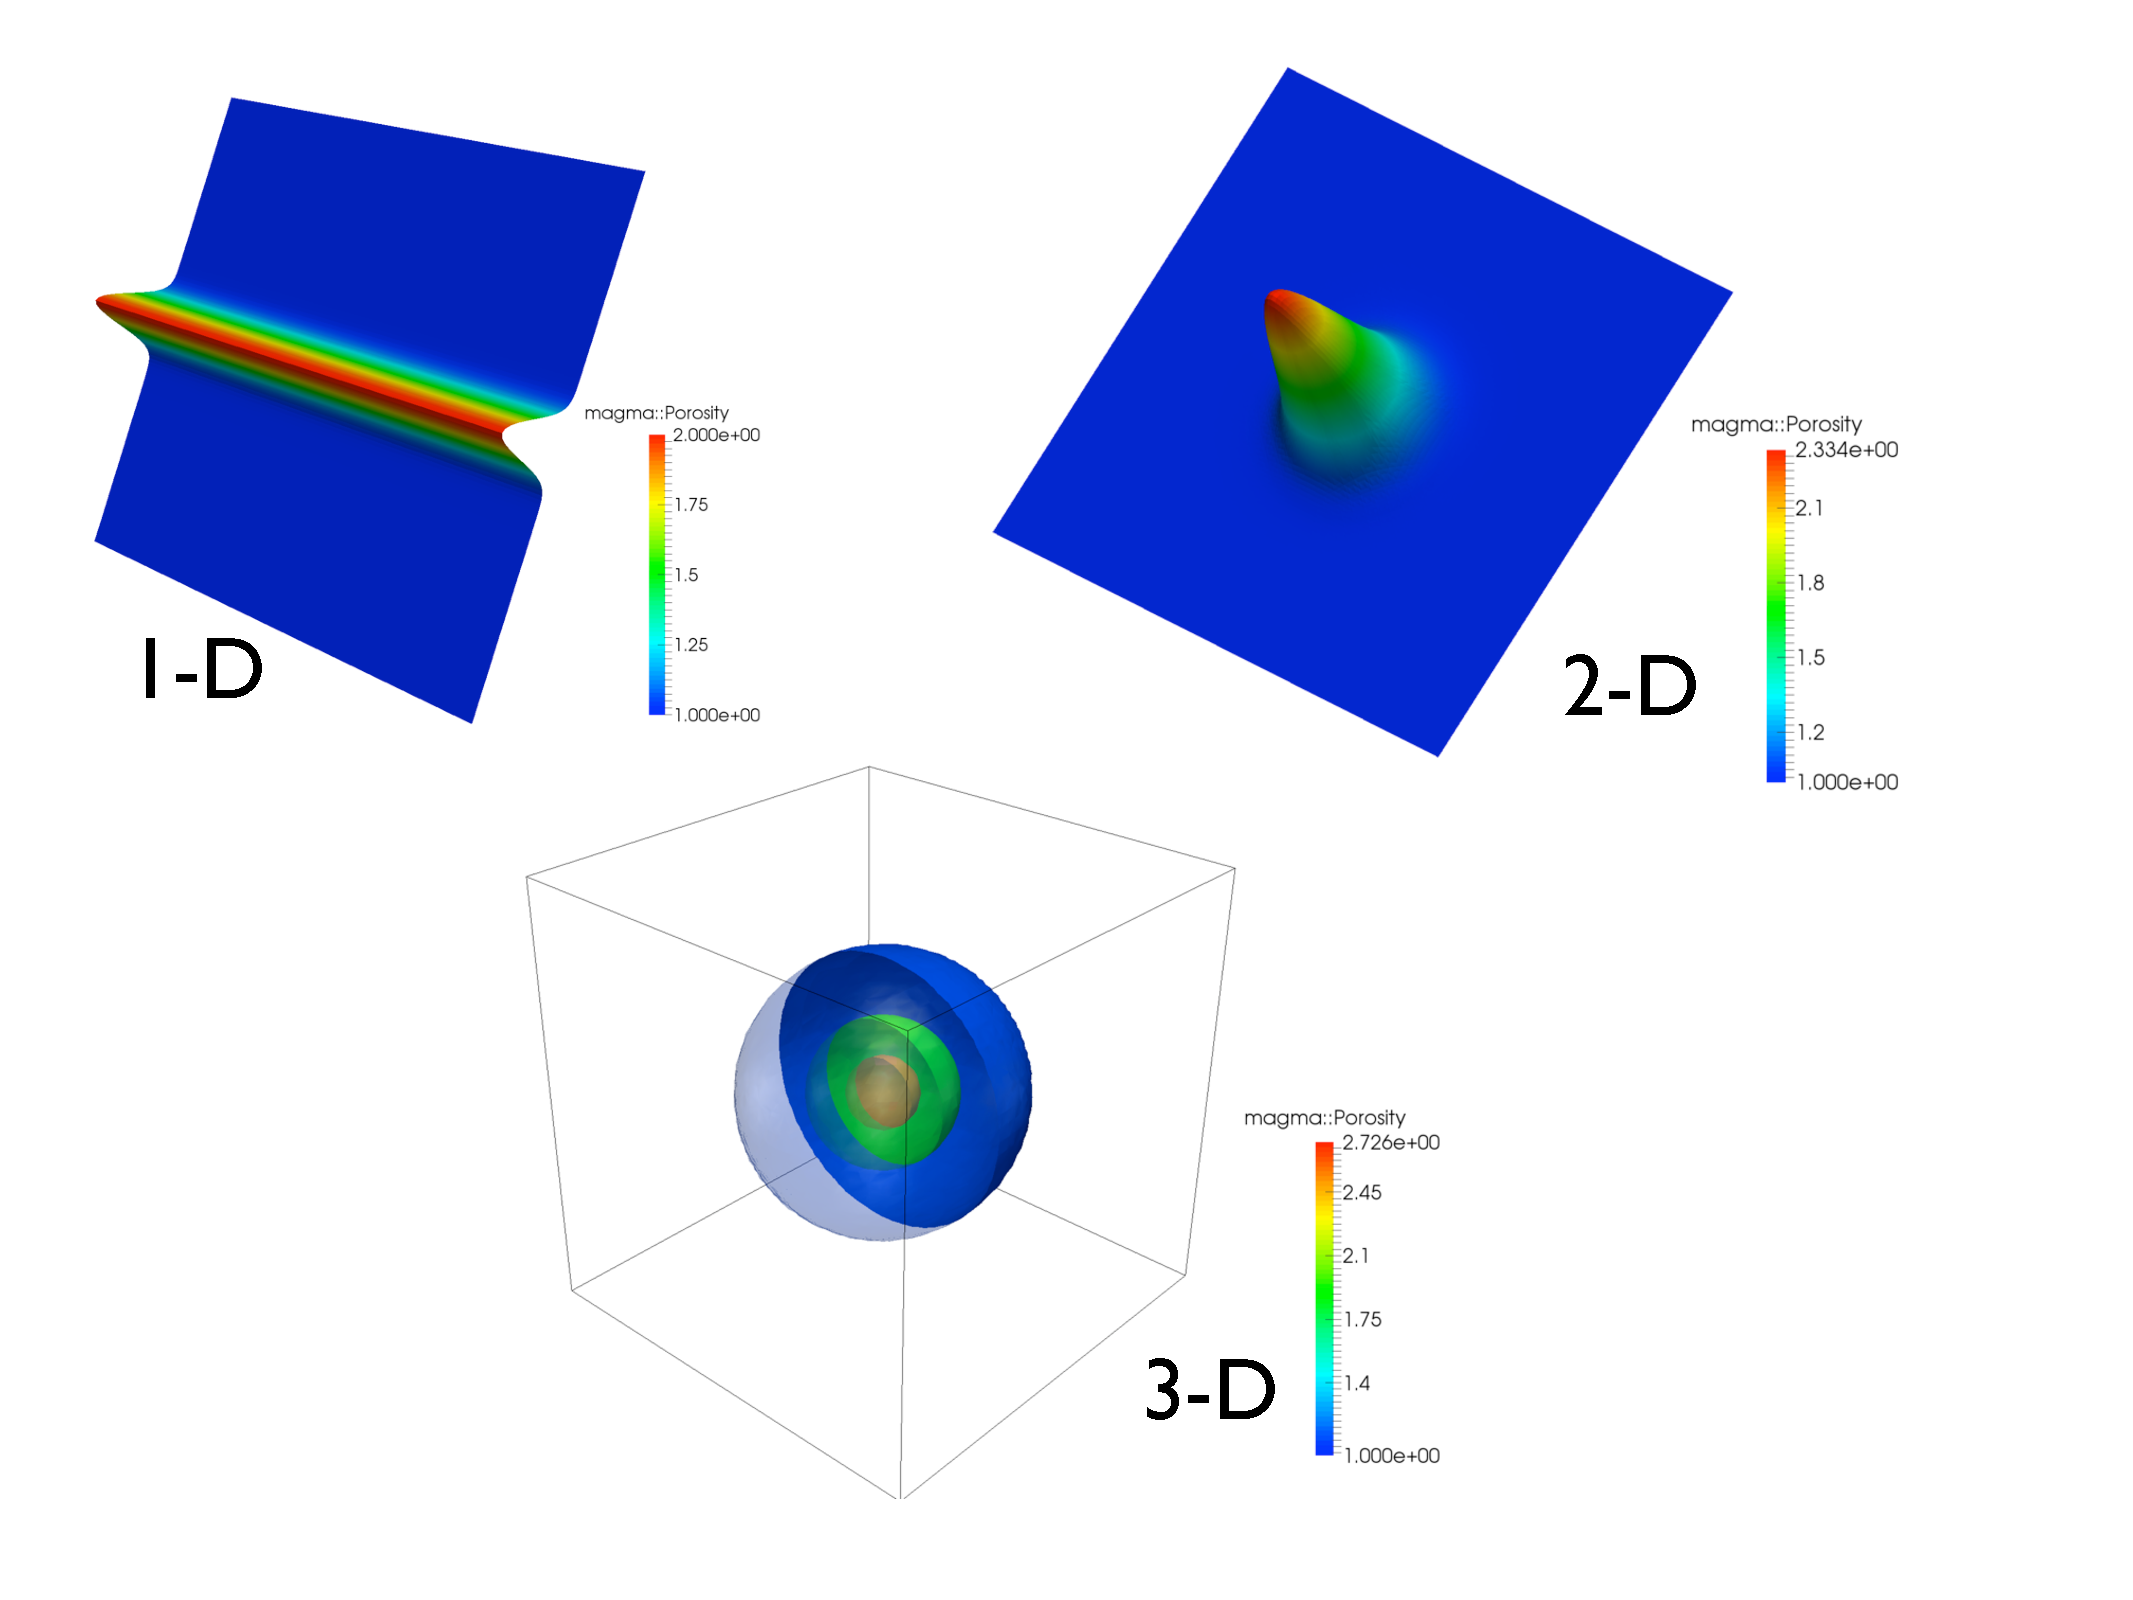
\includegraphics[width=.8\textwidth]{figures/CompositeSolitaryWaves.pdf} 
  \caption{example 1,2 and 3-D magmatic solitary waves that all move
    at speed $c=5$ times the background porosity.}
  \label{fig:SolitaryWavesAllD}
\end{figure}

In the limit of small porosity, the dimensionless governing equations for evolution
of porosity $\phi$ and ``compaction pressure'' $\pcmp$ in a frame
moving at a constant velocity $\Vs$ can be written
\begin{gather}
  \ppt{\phi} + \Vs\cdot\grad\phi = 
  \left(
    \frac{h}{\delta}
  \right)^{2}\frac{\pcmp}{\zeta}  \label{eq:5.1}\\
-\div K \grad\pcmp + \left(
    \frac{h}{\delta}
  \right)^{2}\frac{\pcmp}{\zeta} = \div K \ghat    \label{eq:5.2}
\end{gather}
where $K=\phi^{n}$ is the permeability, $\zeta = 1/\phi^{m}$ is the
bulk viscosity, $\ghat$ is the unit vector in the direction of
gravity.  These equations are scaled by an arbitrary lengthscale $h$
(usually the system height), in which case  $(h/\delta)$ is  the
system height  in compaction lengths
\begin{gather}
  \delta = \sqrt{\frac{K_{0}\zeta_0}{\mu}}
\end{gather}
The compaction length is the intrinsic length scale over which
pressure variations due to obstructions in melt flux propagate as
viscous stresses in the matrix. (See
\cite{spiegelman_flow_1993,spiegelman_flow_1993-1} for more details).

Equations (\ref{eq:5.1})--(\ref{eq:5.2}) for a coupled
hyperbolic/elliptic set of equations for the evolution of porosity and
pressure.  For an arbitrary initial condition, these equations will
break up into a series of localized solitary waves that propagate at a
constant speed that depends on amplitude and maintain constant shape
in the absence of collisions.  Remarkably, however,  we can seek
solitary wave solutions in all dimensions $d$  of the form
\begin{equation}
  \label{eq:5.4}
  \phi(\vec{x},t) = f(r) = f
  \left(
    \sqrt{\sum_{j}^{d-1} x_{j}^{2} + (x_{d} -ct)^{2}}
  \right)
\end{equation}
where $r$ is the radial distance from the peak of the wave.
Substituting $f(r)$ into Equations (\ref{eq:5.1})--(\ref{eq:5.2})
transforms them into a 3rd order, non-linear ODE in $r$.  Except for
some special cases,  these ODE's do not have analytic closed form
solutions, however,  Simpson and Spiegelman
\cite{simpson_solitary_2011}, provides an elegant spectrally accurate
method for numerically calculating solitary wave profiles for all
values of $c,n,m,d$ using the ``sinc collocation method''.  Moreover,
Gideon simpson has encoded this method in a set of python routines
\texttt{magmasinc} which have been included in this tutorial along
with a set of classes for managing and evaluating the solitary wave
profiles.  For example, the script
\texttt{??/??/scripts/see\_solitarywaves.py} initializes 3 different
solitary waves for $c=5$, $n=3$, $m=1$ and $d=[1,2,3]$, using 150
collocation points.  Figure (\ref{fig:SolitaryWaveProfiles}) shows radial profiles $f(r)$ for these
3 waves.  

\begin{figure}[htbp!]
  \centering
  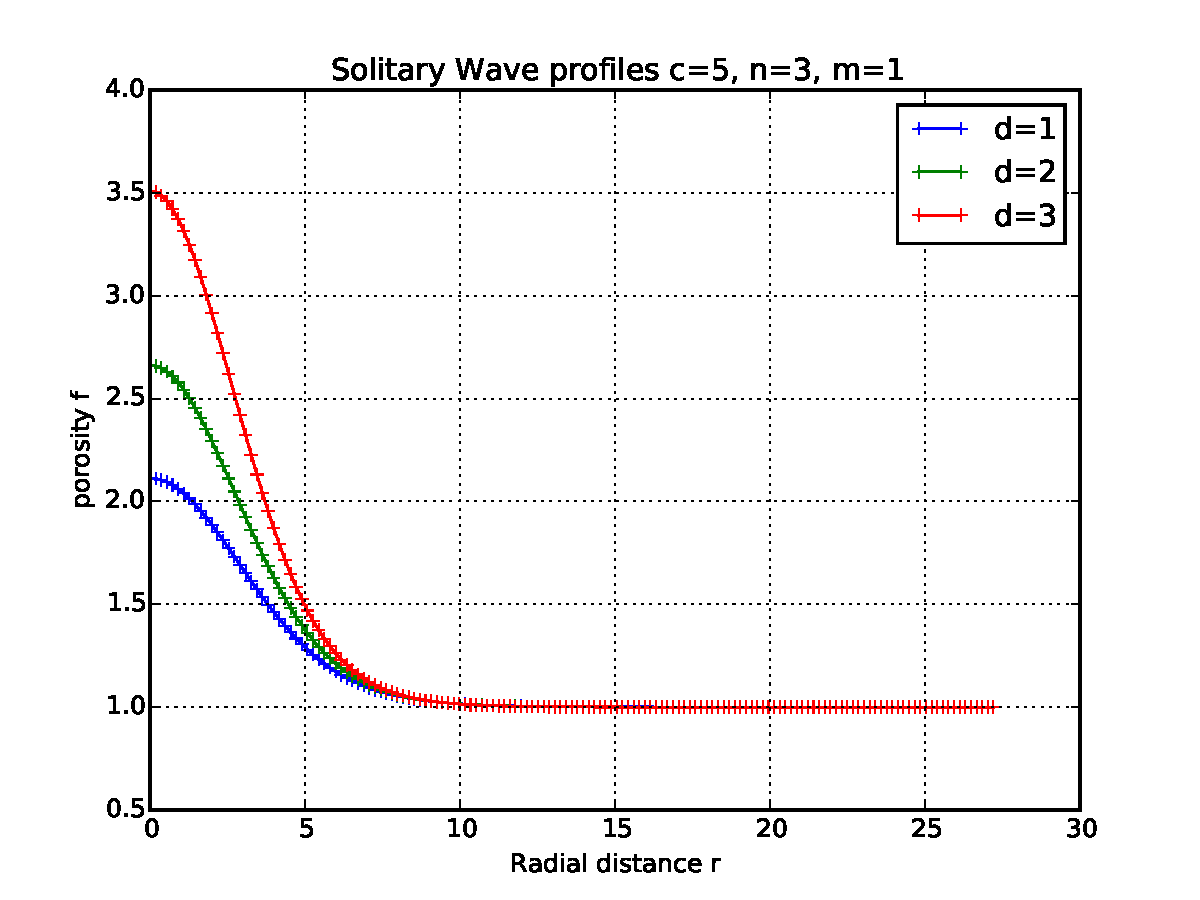
\includegraphics[width=.75\textwidth]{SolitaryWavesProfiles.pdf}
  \caption{Solitary wave profiles $f(r)$ for 1,2 and 3-D waves
    calculated using the pysolwave python package that installs with
    \TF.  All wave travel at speed $c=5$ and have permeability
    exponent $n=3$ and bulk viscosity exponent $m=1$.  Crosses on the
    profiles show the collocation points.}
\label{fig:SolitaryWaveProfiles}
 \end{figure}

\subsection{Benchmark problem}
\label{sec:benchmark-problem}

These solitary waves provide an excellent benchmark problem for
testing any model of multi-phase flow.  If chosen as an initial
condition in a frame moving at speed $\Vs = -c\ghat$ they should
simply stay put and not change shape.  Any error in position or shape
is strictly due to numerical errors.  As a first problem we will
explore the solitary wave benchmarks as laid out in Simpson and
Spiegelman, 2011 \cite{simpson_solitary_2011}. 


\subsection{Variational forms}
\label{sec:variational-forms}



\section{Solution using \TF}
\label{sec:solution-using-tf}



%\pagebreak{}
\section{Themes and Variations}
\label{sec:themes-variations}


\subsection{Variable Viscosity}
\label{sec:variable-viscosity}


%%% Local Variables: 
%%% mode: latex
%%% TeX-master: "tftutorials"
%%% End: 
